% -*- latex -*-
%%%%%%%%%%%%%%%%%%%%%%%%%%%%%%%%%%%%%%%%%%%%%%%%%%%%%%%%%%%%%%%%
%%%%%%%%%%%%%%%%%%%%%%%%%%%%%%%%%%%%%%%%%%%%%%%%%%%%%%%%%%%%%%%%
%%%%
%%%% This text file is part of the lecture slides for
%%%% `Parallel Computing'
%%%% by Victor Eijkhout, copyright 2018-2021
%%%%
%%%% Highercollective-slides.tex : more slides about collective operations
%%%%
%%%%%%%%%%%%%%%%%%%%%%%%%%%%%%%%%%%%%%%%%%%%%%%%%%%%%%%%%%%%%%%%
%%%%%%%%%%%%%%%%%%%%%%%%%%%%%%%%%%%%%%%%%%%%%%%%%%%%%%%%%%%%%%%%

\begin{numberedframe}[containsverbatim]{User-defined operators}
\lstset{language=C}
Given a reduction function:
\begin{lstlisting}
typedef void user_function
    ( void *invec, void *inoutvec, int *len, 
      MPI_Datatype *datatype); 
\end{lstlisting}  
create a new operator:
\begin{lstlisting}
MPI_Op rwz;
MPI_Op_create(user_function,1,&rwz);
MPI_Allreduce(data+procno,&positive_minimum,1,MPI_INT,rwz,comm);
\end{lstlisting}
\end{numberedframe}

\begin{exerciseframe}[onenorm]
  \input ex:one-norm-op
\end{exerciseframe}

\begin{numberedframe}{Non-blocking collectives}
  \label{sl:coll-nonblock-intro}
  \begin{itemize}
  \item Collectives are blocking.
  \item Compare blocking/non-blocking sends:\\
    \indexmpishow{MPI_Send} $\rightarrow$ \indexmpishow{MPI_Isend}
  \item Non-blocking collectives:\\
    \indexmpishow{MPI_Bcast} $\rightarrow$ \indexmpishow{MPI_Ibcast}
  \item Use for overlap communication/computation
  \item Imbalance resilience
  \item Allows pipelining
  \end{itemize}
\end{numberedframe}

\begin{numberedframe}{Use of non-blocking collectives}
  \label{sl:coll-nonblock-use}
  \begin{itemize}
  \item Similar calls, but output a request object:
\begin{lstlisting}
MPI_Isomething( <usual arguments>, MPI_Request *req);
\end{lstlisting}
  \item Calls return immediately;\\
    the usual story about buffer reuse
  \item Requires \lstinline{MPI_Wait}\texttt{...} for completion.
  \item Multiple collectives can complete in any order
  \end{itemize}
\end{numberedframe}

\protoslide{MPI_Ibcast}

\begin{numberedframe}{Overlapping collectives}
  \label{sl:coll-nonblock-overlap}
  Independent collective and local operations:
\[ y \leftarrow Ax + (x^tx)y \]
\begin{lstlisting}
MPI_Iallreduce( .... x ..., &request);
// compute the matrix vector product
MPI_Wait(request);
// do the addition
\end{lstlisting}
\end{numberedframe}

\begin{numberedframe}{Simultaneous reductions}
  \label{sl:coll-nonblock-simult}
  Do two reductions (on the same communicator) with different
  operators simultaneously:
  \[ 
  \begin{array}{l}
    \alpha\leftarrow x^ty\\
    \beta\leftarrow \|z\|_\infty
  \end{array}
  \]
which translates to:
\begin{lstlisting}
MPI_Request reqs[2];
MPI_Iallreduce
   ( &local_xy,  &global_xy, 1,MPI_DOUBLE,MPI_SUM,comm,
     &(reqs[0]) );
MPI_Iallreduce
   ( &local_xinf,&global_xin,1,MPI_DOUBLE,MPI_MAX,comm,
     &(reqs[1]) );
MPI_Waitall(2,reqs,MPI_STATUSES_IGNORE);
\end{lstlisting}
\end{numberedframe}

\begin{exerciseframe}[procgridnonblock]
  \label{sl:coll-nonblock-exgrid}
  \hyperlink{ex:rowcolcomm}{\beamergotobutton{Earlier procgrid exercise}}

  \input ex:procgridnonblock
\end{exerciseframe}

\begin{numberedframe}{Matching collectives}
  \label{sl:coll-nonblock-match}
  Blocking and non-blocking don't match: either all processes
  call the non-blocking or all call the blocking one.
  Thus the following code is incorrect:
\begin{lstlisting}
if (rank==root)
  MPI_Reduce( &x /* ... */ root,comm );
else
  MPI_Ireduce( &x /* ... */ root,comm,&req);
\end{lstlisting}
  This is unlike the point-to-point behavior of non-blocking calls:
  you can catch a message with \indexmpishow{MPI_Irecv}
  that was sent with \indexmpishow{MPI_Send}.
\end{numberedframe}

\begin{numberedframe}{Transpose as gather/scatter}
  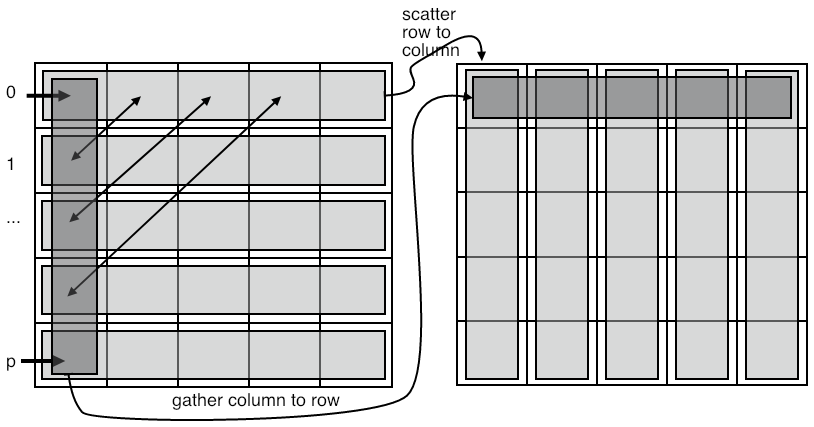
\includegraphics[scale=.3]{alltoall}

  Every process needs to do a scatter or gather.
\end{numberedframe}

\begin{numberedframe}{Simultaneous collectives}
  Transpose matrix by scattering all rows simultaneously.\\
  Each scatter involves all processes, but with a
  different spanning tree.

  \cverbatimsnippet{itransposescatter}
\end{numberedframe}

\begin{numberedframe}{Persistent collectives (MPI-4)}
  Similar to persistent send/recv:
\begin{lstlisting}
MPI_Allreduce_init( ...., &request );
for ( ... ) {
  MPI_Start( request );
  MPI_Wait( request );
}
MPI_Request_free( &request );
\end{lstlisting}
Available for all collectives and neighborhood collectives.
\end{numberedframe}

\begin{numberedframe}{Example}
  \cverbatimsnippet{powerreducepersist}

  Note also the \indexmpishow{MPI_Info} parameter.
\end{numberedframe}

\begin{numberedframe}{Persistent vs non-blocking}
  Both request-based.
  \begin{itemize}
  \item Non-blocking is `ad hoc': buffer info not known before the collective call.
  \item Persistent allows `planning ahead': management of internal buffers and such.
  \end{itemize}
\end{numberedframe}

\begin{comment}
  \begin{numberedframe}{Problem with `progress'}
    \begin{itemize}
    \item Problem: \indexmpishow{MPI_Test} is local
    \item Something needs to force the barrier information to propagate
    \item Solution: force progress with \indexmpishow{MPI_Iprobe}
    \item Frowny face: barrier completion takes much longer than you'd expect.
    \end{itemize}
  \end{numberedframe}
\end{comment}

\sectionframe{Non-blocking barrier}

\begin{numberedframe}{Just what is a barrier?}
  \begin{itemize}
  \item Barrier is not \emph{time} synchronization but \emph{state}
    synchronization.
  \item Test on non-blocking barrier: `has everyone reached some
    state'
  \end{itemize}
\end{numberedframe}

\begin{numberedframe}{Use case: adaptive refinement}
  \begin{itemize}
  \item Some processes decide locally to alter their structure
  \item \ldots~need to communicate that to neighbors
  \item Problem: neighbors don't know whether to expect update calls,
    if at all.
  \item Solution:
    \begin{itemize}
    \item send update msgs, if any;
    \item then post barrier.
    \item Everyone probe for updates, test for barrier.    
    \end{itemize}
  \end{itemize}
\end{numberedframe}

\begin{numberedframe}{Use case: distributed termination detection}
  \begin{itemize}
  \item Distributed termination detection (Matocha and Kamp, 1998):\\
    draw a global conclusion with local operations
  \item Everyone posts the barrier when done;
  \item keeps doing local computation while testing for the barrier to
    complete
  \end{itemize}
\end{numberedframe}

\protoslide{MPI_Ibarrier}

\begin{numberedframe}{Step 1}
  Do sends, post barrier.
\cverbatimsnippet{ibarrierpost}
\end{numberedframe}

\begin{numberedframe}{Step 2}
  Poll for barrier and messages
\cverbatimsnippet{ibarrierpoll}
\end{numberedframe}

\begin{exerciseframe}[ibarrierupdate]
  \begin{itemize}
  \item Let each process send to a random number of randomly chosen
    neighbors. Use \indexmpishow{MPI_Isend}.
  \item Write the main loop with the \indexmpishow{MPI_Test} call.
  \item Insert an \indexmpishow{MPI_Iprobe} call and process incoming messages.
  \item Can you make sure that all sends are indeed processed?
  \end{itemize}
\end{exerciseframe}

\endinput

\begin{numberedframe}{}
\begin{lstlisting}
  
\end{lstlisting}
\end{numberedframe}

